\documentclass[12pt,a4paper]{article}

\usepackage[utf8]{inputenc}
\usepackage[namelimits,sumlimits]{amsmath}
\usepackage{amsfonts,amssymb}
\usepackage{graphicx}
\usepackage{url}
\usepackage{color}
\usepackage{fancyhdr}
% \usepackage{courier}
\usepackage{url}
\usepackage[hmargin=2cm,vmargin=3.2cm,headheight=1cm]{geometry}


% Encadrements
\setlength{\fboxrule}{1.5pt}\setlength{\fboxsep}{2mm}

% De jolis en-têtes
\thispagestyle{fancyplain}
\pagestyle{fancyplain}


\newcommand{\school}{Télécom Physique Strasbourg, TIC-Santé 2ème année}
\renewcommand{\year}{2013-2014}

\lhead[]{\fancyplain{}{\scriptsize\school}}
\rhead[]{}
\lfoot[]{\fancyplain{}{\scriptsize TP de robotique, \year}}
\rfoot[]{\fancyplain{}{O. Kermorgant, B. Bayle}}

% Notations
\newcommand{\ie}{\mbox{\emph{i. e.}}}
\newcommand{\ah}{\mbox{\emph{ad hoc}}}
\newcommand{\ea}{\mbox{\emph{et al.}}}
\newcommand{\cf}{\mbox{\emph{cf.}}}
\newcommand{\etc}{\mbox{\emph{etc.}}}

\renewcommand{\S}{{\cal S}}
\newcommand{\U}{{\cal U}}
\renewcommand{\L}{{\cal L}}
\newcommand{\F}{{\cal F}}
\newcommand{\Z}{{\cal Z}}


\newcommand{\bras}{bras ma\-ni\-pu\-la\-teur}
\newcommand{\brass}{bras ma\-ni\-pu\-la\-teurs}
\newcommand{\pf}{\mbox{plate-forme}}
\newcommand{\pfs}{\mbox{plates-formes}}
\newcommand{\mm}{ma\-ni\-pu\-la\-teur mo\-bi\-le}
\newcommand{\mms}{ma\-ni\-pu\-la\-teurs mo\-bi\-les}
\newcommand{\ot}{\textsc{ot}}
\newcommand{\EO}{\cal M}
\newcommand{\EC}{{\cal N}}

                                % modeles 
\newcommand{\mgd}{\textsc{mgd}}
\newcommand{\mgi}{\textsc{mgi}}
\newcommand{\mcd}{\textsc{mcd}}
\newcommand{\mdd}{\textsc{mdd}}
\newcommand{\mcc}{\textsc{mcc}}
\newcommand{\mcs}{\textsc{mcs}}
                               
                                
                                %situations
\newcommand{\vxi}{\boldsymbol{\xi}}
\newcommand{\derivvxi}{\dot{\vxi}}
\newcommand{\vxiref}{\boldsymbol{\xi}^*}
\newcommand{\derivvxiref}{\dot{\vxi}^*}
\newcommand{\xiun}{\xi_{1}}
\newcommand{\xideux}{\xi_{2}}
\newcommand{\xitrois}{\xi_{3}}
\newcommand{\xiquatre}{\xi_{4}}
\newcommand{\xicinq}{\xi_{5}}
\newcommand{\xisix}{\xi_{6}}
\newcommand{\xim}{\xi_m}

\newcommand{\xun}{x_{1}}
\newcommand{\xdeux}{x_{2}}
\newcommand{\xtrois}{x_{3}}
\newcommand{\xquatre}{x_{4}}
\newcommand{\xcinq}{x_{5}}
\newcommand{\xsix}{x_{6}}
\newcommand{\xm}{x_m}

\newcommand{\vz}{\boldsymbol{z}}
\newcommand{\derivvz}{\dot{\vz}}
\newcommand{\vzp}{\boldsymbol{z}_p}
\newcommand{\derivvzp}{\dot{\vz}_p}

                                %configuration
\newcommand{\vq}{\boldsymbol{q}}
\newcommand{\vqtilde}{\tilde{\vq}}
\newcommand{\derivvq}{\dot{\vq}}
\newcommand{\derivvqtilde}{\dot{\vqtilde}}
\newcommand{\qun}{q_{1}}
\newcommand{\qdeux}{q_{2}}
\newcommand{\qtrois}{q_{3}}
\newcommand{\qquatre}{q_{4}}
\newcommand{\qcinq}{q_{5}}
\newcommand{\qsix}{q_{6}}
\newcommand{\qnu}{q_{\nu}}
\newcommand{\qn}{q_{n}}

\newcommand{\vqp}{{\vq}_p}
\newcommand{\derivvqp}{\dot{\vq}_p}

\newcommand{\vqb}{{\vq}_b}
\newcommand{\derivvqb}{\dot{\vq}_b}
\newcommand{\qbun}{q_{b_1}}
\newcommand{\derivqbun}{\dot{q}_{b_1}}
\newcommand{\qbdeux}{q_{b_2}}
\newcommand{\derivqbdeux}{\dot{q}_{b_2}}
\newcommand{\qbtrois}{q_{b_3}}
\newcommand{\qbquatre}{q_{b_4}}
\newcommand{\qbcinq}{q_{b_5}}
\newcommand{\qbsix}{q_{b_6}}
\newcommand{\qbn}{q_{bn}}
\newcommand{\qbnb}{q_{b_{n_b}}}

\newcommand{\vbeta}{\boldsymbol{\beta}}
\newcommand{\derivvbeta}{\dot{\boldsymbol{\beta}}}
\newcommand{\vphi}{\boldsymbol{\varphi}}
\newcommand{\derivvphi}{\dot{\boldsymbol{\varphi}}}

                                %configuration r�duite
\newcommand{\vp}{\boldsymbol{p}}
\newcommand{\derivvp}{\dot{\vp}}

                                %couples
\newcommand{\vGamma}{\boldsymbol{\Gamma}}
\newcommand{\derivvGamma}{\dot{\vGamma}}
                              
  %vecteur forces generalisees
\newcommand{\vF}{\boldsymbol{F}}
\newcommand{\vFb}{\boldsymbol{F_b}}

                                %erreur
\newcommand{\ve}{\boldsymbol{e}}
\newcommand{\derivve}{\dot{\ve}}

                                %commande
\newcommand{\nbar}{\bar{n}}
\newcommand{\vu}{\boldsymbol{u}}
\newcommand{\derivvu}{\dot{\vu}}
\newcommand{\vup}{\boldsymbol{u}_p}
\newcommand{\vub}{\boldsymbol{u}_b}   
\newcommand{\vus}{\boldsymbol{u}_s}   
\newcommand{\upun}{u_{p_1}}
\newcommand{\updeux}{u_{p_2}}
\newcommand{\nbarp}{\bar{n}_p}
\newcommand{\veta}{\boldsymbol{\eta}}
\newcommand{\vzeta}{\boldsymbol{\zeta}}
\newcommand{\vetap}{\boldsymbol{\eta}_p}
\newcommand{\vzetap}{\boldsymbol{\zeta}_p}
\newcommand{\etap}{\eta_p}
\newcommand{\zetap}{\zeta_p}
\newcommand{\derivvzeta}{\dot{\boldsymbol{\zeta}}}          
\newcommand{\vg}{\boldsymbol{g}}                     
\newcommand{\vn}{\boldsymbol{n}}                     
                                %t�che
\newcommand{\vr}{\boldsymbol{r}}
\newcommand{\derivvr}{\dot{\vr}}

                                %autres
\newcommand{\vb}{\boldsymbol{b}}
\newcommand{\vdf}{\boldsymbol{df}} 
\newcommand{\vf}{\boldsymbol{f}} 
\newcommand{\vfb}{\boldsymbol{f}_b} 
\newcommand{\vm}{\boldsymbol{m}}  
\newcommand{\vs}{\boldsymbol{s}} 
\newcommand{\vx}{\boldsymbol{x}}
\newcommand{\derivvx}{\dot{\vx}}
\newcommand{\vy}{\boldsymbol{y}}
\newcommand{\vX}{\boldsymbol{X}}
\newcommand{\derivvX}{\dot{\vX}}
\newcommand{\vY}{\boldsymbol{Y}}
\newcommand{\derivvY}{\boldsymbol{\dot{Y}}}

                                %t�che additionnelle
\newcommand{\vwa}{{{\boldsymbol{w}}_a}}
\newcommand{\Wa}{W_a(\vqtilde)}
\newcommand{\derivvwa}{\dot{\boldsymbol{w}}_a}

                                %param�tres de Lagrange
\newcommand{\vl}{\boldsymbol{l}}
\newcommand{\vlambda}{\boldsymbol{\lambda}}

 
                                %mgd
\newcommand{\f}{\vf(\vqb, \ \vxip)}
\newcommand{\fb}{\boldsymbol{f}_b(\vq_b)}

                                %Jacobienne en fonction de q
\newcommand{\deltamp}{\delta_{m_p}}
\newcommand{\deltam}{\delta_{m}}
\newcommand{\deltaMp}{\delta_{M_p}}
\newcommand{\deltaM}{\delta_{M}}
\newcommand{\deltasp}{\delta_{s_p}}

\newcommand{\J}{J(\vq)}
\newcommand{\Jun}{J_1(\vq)}
\newcommand{\Junpm}{J_1^{+}(\vq)}
\newcommand{\Jdeux}{J_2(\vq)}
\newcommand{\Jdeuxhatpm}{\hat{J}^{+}_2(\vq)}
\newcommand{\Jdeuxhat}{\hat{J}_2(\vq)}
\newcommand{\Jdeuxpm}{J_2^{+}(\vq)}
\newcommand{\Jt}{J^T(\vq)}
\newcommand{\Jgi}{J^{\#}(\vq)}
\newcommand{\Jstar}{J^{*}(\vq)}
\newcommand{\Jpm}{J^{+}(\vq)}
\newcommand{\Jstarpm}{J^{*+}(\vq)}
\newcommand{\Ja}{J_a(\vq)}
\newcommand{\Jat}{J^T_a(\vq)}
%\newcommand{\Jbar}{\bar{J}(\vq)}      
%\newcommand{\Jbargi}{\bar{J}^{\#}(\vq)}
%\newcommand{\Jbart}{\bar{J}^T(\vq)}   
%\newcommand{\Jbarunpm}{\bar{J}_1^{+}(\vq)}
%\newcommand{\Jbardeux}{\bar{J}_2(\vq)}
%\newcommand{\Jbardeuxhat}{\hat{{\bar{J}}_2}(\vq)}
%\newcommand{\Jbari}{\bar{J}_i(\vq)}   
%\newcommand{\Jbara}{\bar{J_a}(\vq)}   
%\newcommand{\Jbarat}{\bar{J}_a^T(\vq)}

\newcommand{\Jb}{J_b(\vq_b)}
\newcommand{\invJb}{J_b^{-1}(\vq_b)}
\newcommand{\Jbsansq}{J_b}
\newcommand{\Jbt}{J^T_b(\vq_b)}
\newcommand{\Jbtsansq}{J^T_b}
\newcommand{\Jbpm}{J_b^{+}(\vq_b)}
\newcommand{\Jbpmsansq}{J_b^{+}}

\newcommand{\K}{K(\vqb,\ \vartheta)}
\newcommand{\Kun}{K_1(\vqb,\ \vartheta)}
\newcommand{\Kdeux}{K_2(\vqb,\ \vartheta)}
\newcommand{\Kpm}{K^{+}(\vq)}
%\newcommand{\Kbarpm}{\bar{K}^{+}(\vq)}
%\newcommand{\Kbar}{\bar{K}(\vq)}   
%\newcommand{\Kbart}{\bar{K}^T(\vq)}

                                %mcs
%\newcommand{\B}{B(\vqb, \ \vartheta, \ \vbeta_c)}
\newcommand{\Bp}{B_p(\vartheta,\ \vbeta_c)}
\newcommand{\Bun}{B_1(\vqb, \ \vartheta, \ \vbeta_c)}
\newcommand{\Ba}{\boldsymbol{B}_a(\vq)}
\newcommand{\Basansq}{B_a}



\newcommand{\Jbar}{\bar{J}(\vqb, \ \vartheta, \ \vbeta_c)}
\newcommand{\Jbarun}{\bar{J}_1(\vqb, \ \vartheta, \ \vbeta_c)}  
\newcommand{\Jbarex}{\bar{J}(\qbun, \ \qbdeux, \ \vartheta)}
\newcommand{\Jbarcun}{\bar{J}_{C_1}(\vq_{b_1}, \ \vartheta_1, \ \vbeta_{c_1})}
\newcommand{\Jbarsansq}{\bar{J}}
\newcommand{\Jbart}{\bar{J}^T(\vqb, \ \vartheta, \ \vbeta_c)}
\newcommand{\Jbarpm}{\bar{J}^+(\vqb, \ \vartheta, \ \vbeta_c)}
\newcommand{\Jbarunt}{\bar{J}_1^T(\vqb, \ \vartheta, \ \vbeta_c)} 
\newcommand{\Jbartex}{\bar{J}^T(\qbun, \ \qbdeux, \ \vartheta)}
\newcommand{\Jbarpmex}{\bar{J}^+(\qbun, \ \qbdeux, \ \vartheta)}
\newcommand{\Jbartcun}{\bar{J}^T_{C_1}(\vq_{b_1}, \ \vartheta_1, \ \vbeta_{c_1})}
\newcommand{\Jbartsansq}{\bar{J}^T}
\newcommand{\Jbara}{\bar{J}_a(\vq)}
\newcommand{\Jbarasansq}{\bar{J}_a}
\newcommand{\Jbarat}{\bar{J}_a^T(\vq)}
\newcommand{\Jbari}{\bar{J}_i(\vq)}   
\newcommand{\JbarT}{\bar{J}_t(\vq)} 
\newcommand{\JbarTsansq}{\bar{J}_t}
\newcommand{\JbarTt}{\bar{J}_t^T(\vq)}
\newcommand{\JbarTtsansq}{\bar{J}_t^T}
\newcommand{\JbarTpmsansq}{\bar{J}_t^+}
\newcommand{\JbarTpm}{\bar{J}_t^+(\vq)}
\newcommand{\Jbaruntsansq}{\bar{J}_1^T}  
\newcommand{\Jbarunsansq}{\bar{J}_1}  

\newcommand{\dfdqb}{\frac{\partial \vf}{\partial \vqb} (\vqb, \ \vartheta)}
\newcommand{\dfdxip}{\frac{\partial \vf}{\partial \vxip} (\vqb, \ \vartheta)}
                                % mcc

\newcommand{\Spvarthe}{S_p(\vartheta)}
\newcommand{\matS}{S(\vq)}
\newcommand{\Sbar}{\bar{S}(\bar{\vq})}
\newcommand{\Stilde}{\tilde{S}(\vqtilde)}
\newcommand{\Stildesansq}{\tilde{S}}
\newcommand{\Stildepm}{\tilde{S}^{+}(\vqtilde)}
\newcommand{\Stildepmsansq}{\tilde{S}^{+}}
\newcommand{\Stildetsansq}{\tilde{S}^{T}}
\newcommand{\Sbarpm}{\bar{S}^+(\bar{\vq})}
\newcommand{\Sp}{S_p(\vartheta, \ \vbeta_c, \ \vbeta_d)}
\newcommand{\matSsansq}{S}                               
                                %contraintes non holonome
\newcommand{\G}{G(\vq)}
\newcommand{\Gvarthe}{G(\vartheta)}
\newcommand{\Gp}{G_p(\vq_p)}
\newcommand{\Gpvarthe}{G_p(\vartheta)}
\newcommand{\Gt}{G^T(\vq)}
                                % autres (obsoletes...)

\newcommand{\C}{C(\vq)}
\renewcommand{\L}{L(\vq)}
\newcommand{\Lsansq}{L}
\newcommand{\M}{M(\vartheta)}
\newcommand{\E}{\mathsf{E}}
\newcommand{\ZERO}{\mathsf{O}}
                                %svd
\newcommand{\Ub}{U_b(\vq_b)}
\newcommand{\Ubt}{U_b^T(\vq_b)}
\newcommand{\Ubsansq}{U_b}
\newcommand{\Ubtsansq}{U_b^T}
\newcommand{\Vb}{V_b(\vq_b)}
\newcommand{\Vbt}{V_b^T(\vq_b)}
\newcommand{\Vbsansq}{V_b}
\newcommand{\Vbtsansq}{V_b^T}
\newcommand{\Sigmab}{\Sigma_b(\vq_b)}
\newcommand{\Sigmabsansq}{\Sigma_b}
\newcommand{\Sigmabpm}{\Sigma_b^+(\vq_b)}
\newcommand{\Sigmabpmsansq}{\Sigma_b^+}
\newcommand{\Sigmabt}{\Sigma_b^T(\vq_b)}
\newcommand{\sigmabun}{\sigma_{b_1}}
\newcommand{\sigmabdeux}{\sigma_{b_2}}
\newcommand{\sigmabi}{\sigma_{b_i}}
\newcommand{\sigmabm}{\sigma_{b_m}}
\newcommand{\sigmabmb}{\sigma_{b_{m_b}}}
                             
\newcommand{\wb}{w_b}
\newcommand{\wbdeux}{w_{b_2}}
\newcommand{\wbtrois}{w_{b_3}}                  
\newcommand{\wbquatre}{w_{b_4}}
\newcommand{\wbcinq}{w_{b_5}}       

   %rep�res
\newcommand{\R}{{\cal R}}
\newcommand{\Rn}{{\cal R}_n}
\newcommand{\Rprim}{{\cal R}'}
\newcommand{\Rzero}{{\cal R}_0}
\newcommand{\Rsix}{{\cal R}_6}



                                %potentiel
\newcommand{\Pot}{\mathcal{P(\vq)}}
\newcommand{\Pottilde}{\tilde{\mathcal{P}}(\vqtilde)}
\newcommand{\Potsansq}{\mathcal{P}}
\newcommand{\Pottildesansq}{\tilde{\mathcal{P}}}
\newcommand{\Potbtildesansq}{\tilde{\mathcal{P}}_b}
\newcommand{\derivPot}{\mathcal{\dot{P}(\vq)}}
\newcommand{\Pottildeb}{\tilde{\mathcal{P}}_b(\vq_b)}
\newcommand{\Potpb}{\Pottildesansq_{p+b}(\vq)}
\newcommand{\Pottildepb}{\Pottildesansq_{p+b}(\vqtilde)}
\newcommand{\Pottildepbsansq}{\Pottildesansq_{p+b}}

                                %contraintes
\newcommand{\CC}{\overset{\longrightarrow}{C_1C_2}}
\newcommand{\CCabs}{||\CC||}


                                % divers
\newcommand{\fonctionalpha}{\alpha(\vxiref)}
\newcommand{\reals}{\mbox{I \hspace{-3.4mm} R}}

\newcommand{\vgx}{\underline{x}}
\newcommand{\vgy}{\underline{y}}
\newcommand{\vgz}{\underline{z}}
\newcommand{\vgOmega}{\underline{\Omega}}
\newcommand{\vge}{\underline{e}}
\newcommand{\vgvarepsilon}{\underline{\varepsilon}}
\newcommand{\vgp}{\underline{p}}
\newcommand{\vgdp}{\underline{dp}}
\newcommand{\vgdphi}{\underline{d\varphi}}

\newcommand{\Rdeux}{\mathbb{R}^2}
\newcommand{\Rtrois}{\mathbb{R}^3}
\newcommand{\Rtroistrois}{\mathbb{R}^{3 \times 3}}


%%% Local Variables: 
%%% mode: plain-tex
%%% TeX-master: "}"
%%% End: 

\def\vpV{\texttt{vpColVector}}
\def\vpM{\texttt{vpMatrix}}

\begin{document}

\graphicspath{{figs/}}



\vspace{1cm}
\begin{center}
  \fbox{\Large \textbf{TP de robotique - Introduction à ROS}}
\end{center}
\medskip

\section{Objectif} 

\hspace{12pt} L'objectif de ce TP est de contrôler les mouvements d'un robot manipulateur dans l'espace. Pour cela la première étape est le calcul du modèle géométrique direct (MGD) qui donne la position de l'effecteur en fonction des variables articulaires. 
La jacobienne du robot sera ensuite calculée. Une fois ces deux modèles déterminés, le robot pourra être programmé pour suivre une trajectoire, ou bien pour suivre des consignes en vitesse.\\ 

La mise en pratique des modèles et des lois de commande s'appuie sur l'architecture ROS\footnote{ Robot Operating System - http://www.ros.org}. 

\section{Travail préliminaire}

\medskip L'étude porte sur un robot dont le schéma est donné  à la figure
\ref{fig:2RP}. 
\begin{figure}[h]
  \centering
  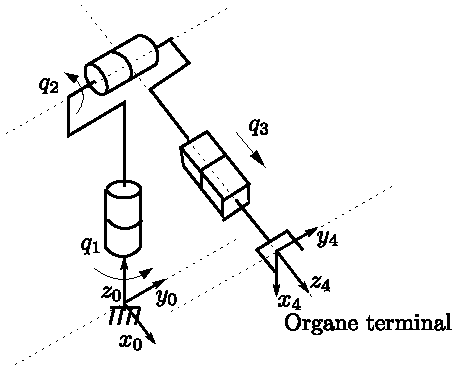
\includegraphics[width=.5\linewidth]{figs/fig-tourelle.pdf}
  \caption{Schéma du robot}
  \label{fig:2RP}
\end{figure}

\vspace*{2cm}

  On adopte la convention des paramètres de
  Denavit-Hartenberg modifiés. On note $T_{i,j}$ la matrice de transformation homogène
  entre les repères $\R_i$ et $\R_j$  et $R_{i,j}$ la matrice de
  rotation entre les repères $\R_i$ et $\R_j$.  On associe à l'organe terminal un repère, noté ${\cal R}_4$, dont l'origine ${\cal O}_4$ a pour coordonnées  $x_1, \ x_2 $
  et $x_3$  (centre de la pince figurée) dans
  ${\cal R}_0$. L'orientation de l'organe terminal est définie par la
  matrice de rotation~:
  \begin{equation*}
    R_{0,3}=R_{0,4}=
    \begin{pmatrix}
      x_{x} & y_{x} & z_{x} \\
      x_{y} & y_{y} & z_{y} \\
      x_{z} & y_{z} & z_{z}
    \end{pmatrix}
  \end{equation*}
  entre ${\cal R}_0$ et ${\cal R}_4$.
  

\begin{itemize}
  
%   \medskip\item[\textbf{\underline{Q1}}] Comment peut-on qualifier le
%   robot manpulateur représenté à la figure \ref{fig:2RP} ?
%   Pour répondre, on se demandera quelle est la forme de l'espace de
%   travail d'un tel robot.
%   
%   \medskip\item[\textbf{\underline{Q2}}] Ce robot, dessiné comme à la figure, s'apparente à un robot tourelle (comme un canon de char...). Utilisé "à l'envers", dans quelle application médicale un robot doté de telles mobilités vous semblerait-il utile ? En manque d'idées, on réfléchira notamment à l'existence d'un point fixe dans le mécanisme.
%   
  \medskip\item[\textbf{\underline{Q1}}] Dessiner le robot dans sa configuration la plus simple et
  placer les repères selon la convention des paramètres de Denavit-Hartenberg modifiés.

  \medskip\item[\textbf{\underline{Q2}}] On note $b$ la distance de la
  base (hachures) à l'axe de la deuxième liaison et  $d$ la distance de l'axe de la deuxième liaison au centre de
  l'organe terminal (centre pince) pour $q_3=0$. On a : $b=0,5 \ m$ et  $d=0,1 \ m$.
  Établir la situation (position + orientation) de l'effecteur en fonction de $(q_1,q_2,q_3)$.
  
  Vérifier pour trois jeux de variables articulaires que le modèle calculé est convenable.

  \medskip\item[\textbf{\underline{Q3}}] Une fois le modèle géométrique direct validé, déterminer le modéle géométrique inverse (MGI) permettant de retrouver le jeu de variables articulaires correspondant à une situation donnée de l'effecteur. Les limites des différentes articulations sont :
  \begin{equation*}
  \begin{array}{ccc}
  q_1\in[-\pi,\pi] & q_2 \in [-1.2,1.2] & q_3\in[0,0.04]
  \end{array}
  \end{equation*}
  
  \medskip\item[\textbf{\underline{Q4}}] Calculer de deux façons différentes la matrice jacobienne du robot.
  
\end{itemize}



\section{Première séance}

\hspace{12pt}La première séance du TP est sous forme de cours intégré et permet de découvrir le fonctionnement de ROS et de faire des rappels de C++ et d'utilisation de la console Unix. On utilisera l'environnement de développement Qt Creator et la bibliothèque mathématique ViSP\footnote{ Bibliothèque dédiée à l'asservissement visuel - http://www.irisa.fr/lagadic/visp}.

ROS, développé par Willow Garage\footnote{ Entreprise créée par des anciens du Stanford Artificial Intelligence Lab}, permet d'interfacer très simplement des logiciels pouvant être écrits par des personnes différentes et dans des langages différents.
Le but de son développement est de pouvoir mettre à disposition de chacun des briques permettant de construire un système complexe.
À titre d'exemple, il existe des briques très performantes pour la vision, la plannification de trajectoire, la cartographie automatique, la commande avancée...

De façon assez logique, les logiciels utilisant ROS se présentent sous une forme élémentaire, le package. Sur un ordinateur donné, tous les packages de l'utilisateur sont situés dans le même dossier.

Pour ce TP nous utilisons l'avant-dernière version de ROS : \emph{Fuerte}. La nouvelle version, \emph{Groovy}, change quelques outils graphiques. La version \emph{Hydro} venait de sortir au moment de la création du TP.

\subsection{Préparation de l'environnement de travail}

\def\bin{<binôme>}

\begin{enumerate}
 \item Une fois connecté sur le PC, ouvrir une console\footnote{ L'utilisation de la console Unix est rappelée en Annexe \ref{anx:unix}} et aller dans le répertoire \texttt{\url{~}/ros\_workspace}.\\
 Il s'agit du répertoire de travail de ROS, tous les paquets de ce répertoire seront donc détectés automatiquement pour la compilation et l'exécution.
Toutes les commandes du TP sont à entrer dans un terminal en ligne de commande.
 \item Aller dans le répertoire \texttt{tpRobots} : 
 \begin{itemize}
  \item \texttt{cd tpRobots} (depuis \texttt{\url{~}/ros\_workspace})
  \item ou plus simplement \texttt{roscd tpRobots} (depuis n'importe où)
 \end{itemize}
 Ce package contient les simulateurs utilisés pour le TP. Pour le mettre à jour et initialiser l'environnement de la machine :
 \begin{itemize}
 \item \texttt{git pull}\footnote{git est un outil de contrôle de version, semblable à svn.}
 \item \texttt{rosrun tpRobots configure.py}
 \end{itemize}
 Afficher ce répertoire dans le gestionnaire de fichiers afin de voir la structure typique d'un package ROS :
 \begin{itemize}
 \item Fichiers à personnaliser par l'utilisateur
 \begin{itemize}
 \item \texttt{manifest.xml} : indique les dépendances à d'autres packages ROS
 \item \texttt{CMakeLists.txt} : indique les sources C++ à compiler
 \end{itemize} 
 \item Dossiers créés par l'utilisateur :
 \begin{itemize}
 \item \texttt{src} : fichiers source (ici en C++ et Python)
 \item \texttt{include} : headers des fichiers C++
 \item \texttt{launch} : contient les fichiers \emph{launchfile} qui automatisent l'exécution de plusieurs programmes à la fois
 \item \texttt{urdf} : contient les fichiers urdf (Universal Robot Description File), décrivant les modèles géométriques des robots
 \end{itemize}
 \item Dossiers créés automatiquement à la compilation (peuvent ne pas être présents)
 \begin{itemize}
 \item \texttt{bin} : exécutables compilés
 \item \texttt{build} : fichiers temporaires de compilation
 \item \texttt{lib} : librairie compilée
 \end{itemize}
 \end{itemize}
 
 \item Effacer les dossiers créés automatiquement puis compiler le package :
 \begin{itemize}
 \item \texttt{rm -rf bin build lib} 
 \item \texttt{rosmake tpRobots}
 \end{itemize}
 \end{enumerate}
 
 \subsection{Nodes et topics}
 
\begin{enumerate}

\item On voit qu'un exécutable \texttt{simu4Points} a été compilé dans \texttt{bin}. Dans ROS les exécutables sont appelés des \emph{nodes}.
ROS intègre la complétion automatique. Pour exécuter un node, taper :
\begin{itemize}
\item \texttt{rosrun tp<tab>} : complète avec le nom du package
\item \texttt{rosrun tpRobots <tab>} : indique les nodes disponibles
\end{itemize}
La commande \texttt{rosrun} est juste un raccourci pour exécuter les programmes se trouvant dans un package ROS avec l'aide de l'autocomplétion. Cela permet de lancer des programmes se trouvant dans différents dossiers sans avoir besoin de naviguer dans le système de fichiers.

On voit qu'en plus de \texttt{simu4Points}, ROS nous propose d'exécuter \texttt{arm\_bridge.py}, \\\texttt{configure.py}  et \texttt{setpoint4Points.py}. Il s'agit de fichiers Python qui n'ont pas besoin d'être compilés pour être lancés\footnote{ Pour être détecté par \texttt{rosrun} un fichier Python doit être exécutable}.
On reconnaît le fichier \texttt{configure.py} qui a été lancé au début pour initialiser l'environnement.
\item Dans la prise en main nous nous intéressons à :
\begin{itemize}
\item  \texttt{simu4Points} : simule un asservissement visuel
\item \texttt{setpoint4Points.py} : génère des consignes de position
\end{itemize}
 Ces deux programmes doivent pouvoir communiquer entre eux si on veut que l'un suive les consignes de l'autre.
Essayer d'exécuter chacun des programmes (dans une console différente) pour observer qu'ils attendent la présence d'un "master".
Il s'agit du logiciel ROS chargé de mettre en relation les différents nodes : le lancer via la commande \texttt{roscore} (dans un nouveau terminal).
Les deux nodes se lancent aussitôt.
\item Dans une nouvelle console, exécuter \texttt{rxgraph}  pour observer la structure élémentaire de l'architecture ROS :
\begin{itemize}
\item Les nodes se sont enregistrés sous les noms \texttt{/SetpointGenerator} et \texttt{/Main\_control} 
\item Le premier envoie un message appelé \texttt{/setpoint} au second : ce canal de communication est appelé un \emph{topic}
\end{itemize}
Indépendamment du langage, utiliser ROS revient essentiellement à mettre en relation des programmes élémentaires qui souscrivent et publient chacun des informations sur différents topics.
\begin{itemize}
\item Publier : déclarer au ROSmaster qu'on va envoyer des informations sur un topic, sans s'intéresser à la destination de ces données
\item Souscrire : déclarer au ROSmaster qu'on est intéressé par ce qui se passe sur un topic donné, sans s'intéresser à la source de ces données
\item Plusieurs nodes peuvent souscrire et publier sur le même topic : importance de se mettre d'accord pour éviter les embouteillages
\end{itemize}
Le ROSmaster se charge de mettre les nodes en relation. Une architecture typique peut être :
\begin{itemize}
\item Un node interfacé avec une caméra, faisant l'aquisition des images et les publiant sur un topic
\item Un node chargé de récupérer ces images, les traiter et publier la position d'un objet d'intérêt
\item Un node récupérant ces positions et calculant la consigne à effectuer pour atteindre l'objet
\item Un node interfacé avec un robot, qui ne fait qu'appliquer les consignes de position qu'il reçoit sur le topic auquel il souscrit
\end{itemize}
Chaque node pouvant être codé, exécuté et compilé indépendamment, cela permet une grande souplesse pour le développement de systèmes complexes.

\end{enumerate}
\subsection{ROS dans le code}
\begin{enumerate}
\item On a pu voir que ROS disposait de nombreux outils en ligne de commande\footnote{ Ces outils sont résumés en Annexe \ref{sec:lignecomm}}.
Pour pouvoir exploiter ces avantages dans le logiciel Qt Creator, il faut également le lancer depuis une console : \texttt{qtcreator}.
Lors des prochaines séances il faudra également lancer Qt Creator via la console\footnote{ Attention notamment à l'ouverture automatique des \texttt{.cpp} dans Qt Creator : le logiciel ainsi lancé ne sera pas interfacé avec l'environnement ROS.}.
Pour ouvrir le package tpRobots :
\begin{itemize}
\item Avec \texttt{File/Open file}, choisir le fichier \texttt{CMakeList.txt} du package tpRobots
 \item Indiquer \texttt{tpRobots/build} comme répertoire de compilation
 \item Valider et exécuter CMake pour obtenir l'affichage des fichiers source
 \item Avec \texttt{File/Open file}, ouvrir également le fichier \texttt{src/setpoint4Points.py}
\end{itemize}
\item Parcourir les fichiers \texttt{simu4Points.cpp} et \texttt{setpoint4Points.py} pour y repérer les lignes propres à ROS : déclaration du nom du node, souscription et publication des topics. On voit apparaître la notion de message : il s'agit du type d'information que des nodes s'échangent sur un topic (vecteur, image, chaîne de caractère...). Ici le message \texttt{/setpoint} est un \texttt{Float32MultiArray}, soit un vecteur de float. De nombreux types de message existent déjà dans ROS, mais il est toujours possible de créer le sien pour une utilisation particulière.

On peut noter à la fin de \texttt{simu4Points.cpp} que ce node publie les positions et les erreurs de position. Ces topics ne sont écoutés par aucun node. 
Ce node publie également les images acquises par le robot, sur le topic \texttt{/camera/image}. 
Heureusement il n'y a pas besoin d'aller lire du code pour connaître les topics disponibles.
Des outils en ligne de commande existent pour analyser les informations circulant sur les topics.

\end{enumerate}
\subsection{Outils sur les topics - rostopic}
\begin{enumerate}

\item La commande \texttt{rostopic} permet de manipuler les topics via la console :
\begin{itemize}
\item \texttt{rostopic list} : liste les topics actifs
\item \texttt{rostopic echo <topic>} : affiche le contenu d'un topic
\item \texttt{rostopic info <topic>} : donne des infos sur un topic (nodes publiant et souscrivant, type de message)
\end{itemize}
Vérifier la présence des autres topics publiés.
\item Si le topic contient des valeurs numériques, ce qui est le cas des \texttt{Float32MultiArray}, \texttt{rxplot} peut en tracer la courbe temporelle : 
\begin{itemize}
\item Commande : \texttt{rxplot <topic>/<attribut>[indice] -p <intervalle de temps>}
\item Par exemple : \texttt{rxplot setpoint/data[0] -p 10}
\end{itemize}
\item Si le topic contient des images, un outil permet de les afficher. Vérifier que le topic \texttt{camera/image} contient des données de type \texttt{sensor\_msgs/Image} puis les afficher :
\begin{itemize}
\item \texttt{rosrun image\_view image\_view image:=camera/image}
\end{itemize}
On reconnaît la syntaxe ROS : \texttt{image\_view} est un node du package lui aussi appelé \texttt{image\_view}. Ce node prend en argument le topic sur lequel recevoir des images pour simplement les afficher dans une fenêtre. Dans notre cas, le node de simulation a aussi sa propre fenêtre : il réalise l'opération inverse, à savoir publier sur un topic les images générées.
\end{enumerate}

\subsection{Serveur de paramètres - rosparam}

Le ROSmaster inclue également un serveur de paramètres. Tous les nodes peuvent ainsi récupérer et écrire des valeurs diverses et variées.
Les paramètres sont à utiliser de préférence aux topics pour communiquer des valeurs qui changent peu souvent et qui n'ont pas besoin d'être diffusées à chaque itération sur le réseau.

On peut ainsi voir que \texttt{setpoint4Points.py} utilise Ts (période des créneaux pour les consignes) comme un paramètre. L'intérêt est aussi de pouvoir modifier les paramètres en ligne de commande pendant que les programmes tournent :
\begin{itemize}
\item \texttt{rosparam list} : liste les paramètres disponibles
\item \texttt{rosparam get Ts} : affiche la valeur de \texttt{Ts}
\item \texttt{rosparam set Ts 1} : met à jour le paramètre
\end{itemize}
De la même façon, \texttt{simu4Points.cpp} indique que le gain \texttt{Kp} de la loi de commande est un paramètre.
Utiliser cet outil avec \texttt{Ts} et \texttt{Kp} pour changer la période des consignes et le gain de l'asservissement.

\subsection{Gérer les exécutions simultanées - roslaunch}

Pour un robot complexe il peut rapidement y avoir plusieurs nodes à exécuter et plusieurs paramètres à initialiser afin que tout tourne correctement. Le lancement simultané de plusieurs nodes est géré par l'outil \texttt{roslaunch} :
\begin{itemize}
\item \texttt{roslaunch <package> <launchfile>} : exécute le launchfile
\end{itemize}
Quitter les nodes ainsi que le \texttt{roscore}.
Ouvrir le fichier \texttt{tpRobots/launch/sim.launch} afin de constater qu'il initialise les deux paramètres \texttt{Ts} et \texttt{Kp} et qu'il lance les deux nodes \texttt{setpoint4Points.py} et \texttt{simu4Points}.
L'exécuter et vérifier que la simulation fonctionne : \texttt{roslaunch} lance automatiquement le ROSmaster s'il n'est pas déjà actif.

\subsection{Enregistrer et rejouer des données - rosbag}
La commande \texttt{rosbag} permet de sauvegarder dans un fichier tout ou partie des données circulant sur les topics.
\begin{enumerate}

\item Pour enregistrer l'ensemble des topics : 
\begin{itemize}
\item \texttt{rosbag record -a} : crée un fichier binaire \texttt{.bag} avec les contenus des topics.
\end{itemize}
Arrêter l'enregistrement après quelques dizaines de secondes, et quitter les deux nodes (\texttt{Ctrl-C} dans les consoles).
\item Deux outils existent pour relire les topics :
\begin{itemize}
\item \texttt{rosbag play <fichier.bag>} : republie les données sur les topics enregistrés
\item \texttt{rxbag <fichier.bag>} : ouvre une interface permettant de choisir les topics republiés
\end{itemize}
Relancer le ROSmaster. Avec \texttt{rxbag}, lancer la republication de \texttt{/setpoint}.
Relancer le node \texttt{simu4Points} : noter qu'il suit la consigne alors que le node \texttt{setpoint4Points} n'est pas lancé. En effet les consignes enregistrées sont republiées sur le même topic. Le node ne s'intéresse pas à la source du topic, seulement à son contenu. 

\item Noter que  \texttt{simu4Points} a recommencé à publier ses topics. Que se passe-t-il si avec \texttt{rxbag} on lance la publication parallèle d'un même topic, par exemple \texttt{/position}  ? Utiliser \texttt{rxplot} pour visualiser l'effet d'un conflit de publication (plusieurs nodes publiant sur le même topic sans se concerter).
\end{enumerate}

\subsection*{Pour approfondir}

Des tutoriaux pour bien d'autres aspects de ROS sont disponibles en ligne
\begin{itemize}
\item \texttt{http://wiki.ros.org/ROS/Tutorials}
\end{itemize}



\newpage
\section{Deuxième séance}
La deuxième séance est consacrée à la modélisation du robot.
Pour cela un package sera créé par le binôme. 
\begin{enumerate}
 \item  Création d'un package personnel : retourner dans le répertoire \texttt{\url{~}/ros\_workspace}. On souhaite y créer un package qui sera dépendant de \texttt{tpRobots}
  \begin{itemize}
   \item Création du package : \texttt{roscreate-pkg \bin ~tpRobots}
   \item Copier le fichier \texttt{tpRobots/src/control.cpp} dans le nouveau package
   \item Modifier le fichier \texttt{\bin/CMakeLists.txt} pour indiquer à ROS de compiler la source : \\
   \texttt{rosbuild\_add\_executable(control control.cpp)}
  \end{itemize}
  \item Ouverture du package personnel dans Qt Creator
  \begin{itemize}
 \item Taper dans une ligne de commande : \texttt{qtcreator}
 \item Dans \texttt{Fichier/Ouvrir un fichier}, choisir le fichier \texttt{CMakeList.txt} du package personnel
 \item Indiquer \texttt{\bin/build} comme répertoire de compilation
 \item Valider et exécuter CMake pour obtenir l'affichage des fichiers source
\end{itemize}
\end{enumerate}

\subsection{Fonctionnement du node de commande}

Ouvrir le fichier \texttt{control.cpp}. On voit qu'il instancie une classe \texttt{tpRobot} avec un certain nombre de degrés de liberté :
\begin{verbatim}
   // init robot
    const unsigned int N = 3;
    tpRobot robot(rosNH, N);
\end{verbatim}

Cette classe intègre les interfaces (publication et souscription de topics) avec les autres nodes ROS. Elle contient trois méthodes :
\begin{itemize}
 \item \texttt{robot.getPosition(q)} : récupère les valeurs des variables articulaires
 \item \texttt{robot.setPosition(q)} : envoie une consigne de position \texttt{q}
 \item \texttt{robot.setVelocity(v)} : envoie une consigne de vitesse \texttt{v}
\end{itemize}
Les variables \texttt{q} et \texttt{v} sont de classe \vpV, qui est un vecteur au sens mathématique. Son fonctionnement est détaillé en Annexe \ref{sec:visp}. \\

L'objectif du TP est donc d'utiliser la mesure de position articulaire pour calculer le modèle géométrique, et envoyer des consignes de position ou de vitesse au simulateur. Par la suite la programmation se fera en modifiant \texttt{control.cpp}.

\begin{enumerate}
  \item Compilation du package personnel : 
  \begin{itemize}
   \item Sous Qt Creator : icône de marteau en bas à gauche
   \item En ligne de commande : \texttt{rosmake \bin}
   \end{itemize}
     \item Exécution du node personnel
  \begin{itemize}
  \item Sous Qt Creator : icône de triangle vert en bas à gauche
  \item En ligne de commande :  \texttt{rosrun \bin~control}
   \item Sous ROS, le nom de ce node est \texttt{/mainControl}
   \item Il est possible de lancer le programme en mode debug avec le triangle vert surmonté d'un insecte
  \end{itemize}
\end{enumerate}

Les différents nodes et topics interagissant dans le TP sont détaillés en Annexe \ref{sec:nodes}.
Une fois lancé, le node tel qu'il est ne fait qu'attendre la publication des positions articulaires du robot.


\subsection{Visualisation avec RViz} 
  
Compiler et lancer le simulateur : 
 \begin{itemize}
 \item \texttt{roslaunch tpRobots turret3.launch}
 \end{itemize}
 L'interface RViz apparaît avec un modèle 3D.
RViz permet d'afficher la situation globale du robot. La fenêtre de gauche donne des informations sur les différents éléments (links) du robot.
Notamment, comme montré en Fig.\ref{fig:rviz}, il est possible de lire la position et l'orientation de l'effecteur (end\_effector). 
On utilisera donc cette fenêtre pour valider le modèle géométrique.\\
En cochant la case ``Show Trail'', RViz affiche également la trajectoire suivie par l'effecteur.

\begin{figure}[h]\centering
 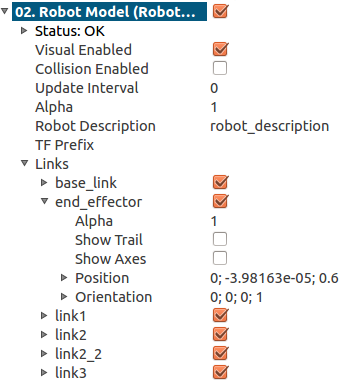
\includegraphics[width=.3\linewidth]{rviz}
 \caption{Lecture de la situation de l'effecteur dans RViz}
 \label{fig:rviz}
\end{figure} 
 
 \subsection{Travail demandé}
 \label{travail2s}

\begin{itemize}
 \medskip\item[\textbf{\underline{Q1}}] Programmer une fonction \texttt{CalcMGD}\footnote{ L'Annexe \ref{anx:cpp} rappelle les différents prototypes de fonction en C++} qui calcule la position opérationnelle en fonction du vecteur des variables articulaires. La fonction est à coder dans \texttt{control.cpp}, avant le \texttt{main()}.
 Afficher dans la console la position ainsi obtenue.


  \medskip\item[\textbf{\underline{Q2}}] En jouant sur les sliders (fenêtre \texttt{Joint State Publisher}), comparer en plusieurs endroits les valeurs de votre programme avec celles indiquées par le simulateur (Fig.\ref{fig:rviz}).
 Valider ainsi le modèle calculé.
 
 \medskip\item[\textbf{\underline{Q3}}] Afficher le graphe des nodes et des topics. Appeler l'encadrant de TP pour décrire le fonctionnement de l'architecture affichée. 
 
 \medskip\item[\textbf{\underline{Q4}}] Programmer une fonction \texttt{CalcMGI} qui calcule le modèle géométrique inverse de façon analytique. 
 Coder la simulation alternant toutes les 10 secondes\footnote{La fréquence en Hz est déjà indiquée dans le code par l'instruction \texttt{ros::Rate loop(30)}. 10 secondes correspondent donc à 300 itérations dans la boucle while.} entre les points $X_1=(-0.065,-0.02,0.61)$ et $X_2=(-0.046, -0.046, 0.6)$.
 

  \medskip\item[\textbf{\underline{Q5}}] Afficher le graphe des nodes et des topics. Sachant que le node \texttt{jointControl} convertit des consignes de position ou de vitesse et publie la position articulaire du robot sur \texttt{/jointControl/position}, commenter sur les conflits possibles avec l'interface des sliders \texttt{/joint\_state\_publisher}.
 
 \medskip\item[\textbf{\underline{Q6}}]  Vérifier dans une console que les positions obtenues sont bien celles demandées :
 \begin{verbatim}
 rosrun tf tf_echo base_link end_effector
\end{verbatim}Valider ainsi le modèle géométrique inverse. 

On pourra aussi créer un nouveau \emph{publisher} (Annexe \ref{sec:publish}) permettant d'afficher avec \texttt{rxplot} l'évolution de l'erreur opérationnelle.

\medskip\item[\textbf{\underline{Q7}}] En cochant la case ``Show Trail'' de l'effecteur sous RViz, commenter la trajectoire obtenue.

\end{itemize}

\newpage

\section{Troisième séance}

La deuxième séance porte sur l'exploitation du jacobien dans la commande. On souhaite maintenant contrôler le robot dans l'espace opérationnel.

\begin{itemize}
 \medskip\item[\textbf{\underline{Q1}}] Programmer une fonction \texttt{CalcJ} qui calcule la matrice jacobienne (classe \texttt{vpMatrix}) en fonction du vecteur des variables articulaires.
 
 \medskip\item[\textbf{\underline{Q3}}] On souhaite toujours que le robot se déplace entre $X_1=(0.065,-0.02,.61)$ et $X_2=(-0.046, -0.046,  0.6)$., mais en allant de point en point de l'espace opérationnel, à l'aide du modèle géométrique inverse.
Programmer cette stratégie, en utilisant l'une ou l'autre des procédure de calcul de MGI.
 Vérifier avec  \texttt{tf} ou  \texttt{rxplot} que les points sont bien atteints.
 
 
 \medskip\item[\textbf{\underline{Q4}}] En cochant la case ``Show Trail'' de l'effecteur sous RViz, commenter la trajectoire obtenue.
 
 \medskip\item[\textbf{\underline{Q5}}] On souhaite réaliser le même mouvement qu'à la question Q3.
 On s'inspirera de la partie 3.2.2 de la seconde partie du cours de Robotique. On fera le mouvement opérationnel à vitesse constante dans un premier temps. Programmer cette procédure, vérifier que les points sont bien atteints et afficher la trajectoire correspondante.
  

 \end{itemize}
 
 \newpage
\section{Pour aller plus loin}
 
 On a pu voir qu'une fois la modélisation géométrique validée, le schéma de commande est sensiblement le même. 

\begin{enumerate}
\item Modéliser le robot suivant :
\begin{figure}[h]
  \centering
  
\includegraphics[width=.4\linewidth]{figs/scara4}
  \caption{Schéma du robot 4 degrés de liberté}
  \label{fig:3RP}
\end{figure}\\
Avec les distances :
\begin{itemize}
\item Hauteur totale : $h=0.27$
\item Longueur premier bras : $a=0.20$
\item Longueur deuxième bras : $b = 0.15$
\item Distance entre l'axe du deuxième bras et le centre de l'effecteur pour $q_4=0$ : $c=0.07$
\end{itemize}
On souhaite contrôler à la fois la position cartésienne de l'effecteur et l'angle pris par le 3ème axe. On note $\tilde{P} = (x,y,z,q_3)$.\\
Pour le contrôleur on n'oubliera pas d'initialiser $N$ à 4.
\item Valider le modèle géométrique avec le simulateur :
\begin{itemize}
\item \texttt{roslaunch tpRobots scara4.launch}
\end{itemize}
\item 
Comme en deuxième séance, utiliser le MGI pour osciller entre les positions $\tilde{P}_1=(0.3,0.1,0.2,0.4)$ et $\tilde{P}_2=(0.3,0.1,0.2,-0.4)$.
Les limites des articulations sont :
  \begin{equation*}
  \begin{array}{cccc}
  q_1\in[-\pi/2,\pi/2] & q_2 \in [-\pi/2,\pi/2] & q_3\in[-\pi/2,\pi/2] & q_4\in[-0.04,0.04]
  \end{array}
  \end{equation*}
\item Calculer la jacobienne associée à $\tilde{P}$. L'utiliser pour réaliser le même mouvement dans l'espace opérationnel. Que dire des trajectoires ?
\end{enumerate}


\appendix

\newpage

\section{Syntaxe Unix}\label{anx:unix}

On rappelle ici quelques éléments de syntaxe de la console Unix.

\begin{itemize}
\item \texttt{cd <répertoire>} : va dans le répertoire indiqué
\item \texttt{ls} : liste les fichiers du répertoire courant
\item \texttt{./<exécutable>} : exécute le programme indiqué 
\item \texttt{Ctrl - C} : annule la commande actuelle, force la fermeture du programme qui a été lancé dans cette console
\item \texttt{Ctrl - Shift - C} : Copie le texte sélectionné
\item \texttt{Ctrl - Shift - V} : Colle le texte sélectionné
\end{itemize}

Même s'il est possible d'avoir plusieurs fenêtre de terminaux, il est parfois moins confus d'avoir plusieurs onglets dans une même fenêtre.
Ces onglets sont gérés comme suit :
\begin{itemize}
\item \texttt{Ctrl - Shift - T} : ouvre un nouvel onglet
\item \texttt{Ctrl - Shift - W} : ferme l'onglet courant
\item \texttt{Ctrl - Shift - Q} : ferme la fenêtre courante et tous ses onglets
\end{itemize}

\section{Rappels de syntaxe C++}
\label{anx:cpp}

On rappelle ici les prototypages standards des fonctions en C++. Le but est de prendre l'habitude de se servir des références ou des objets en fonction de ce qu'on veut faire des arguments d'une fonction.

\begin{itemize}
\item Passage par copie : \texttt{f(vpMatrix M)}
\begin{itemize}
\item La matrice \texttt{M} peut être modifiée dans la fonction
\item Elle ne sera pas modifiée à la sortie : la fonction travaille sur une copie de \texttt{M}
\end{itemize}
\item Passage par référence : \texttt{f(vpMatrix \&M)}
\begin{itemize}
\item La matrice \texttt{M} peut être modifiée dans la fonction
\item Elle sera modifiée également en dehors de la fonction
\item Utile pour des fonctions qui mettent à jour certaines variables
\end{itemize}
\item Passage par référence constante : \texttt{f(const vpMatrix \&M)}
\begin{itemize}
\item La matrice \texttt{M} ne peut pas être modifiée dans la fonction
\item L'appel à la fonction ne mobilise pas de ressources car il n'y a pas de recopie
\item Utile pour des fonctions qui utilisent une variable sans avoir le droit de la modifier
\end{itemize}
\end{itemize}



\section{Outils intégrés à ROS}
\label{sec:lignecomm}

ROS propose plusieurs outils en ligne de commande permettant d'aider le développement et le diagnostic.
\subsection{Outils en ligne de commande}
\begin{itemize}
\item \texttt{roscd <package>} : va dans le répertoire du package
 \item \texttt{rosmake <package>} : compile le package
 \item \texttt{rosrun <package> <program>} : exécute le programme contenu dans le package 
 \item \texttt{rosnode list} : liste les nodes existant
 \item \texttt{rostopic list} : liste les topics existant
 \item \texttt{rostopic echo <topic>} : affiche les données circulant sur le topic
\end{itemize}

\subsubsection*{Matrice de passage}

La valeur courante de la transformation entre l'effecteur et la base s'obtient par : 
\begin{verbatim}
 rosrun tf tf_echo base_link end_effector
\end{verbatim}
\texttt{tf} est le package de ROS gérant la correspondante entre les variables articulaires et les matrices de transformation. 
\texttt{tf\_echo} est un node de ce package qui se contente d'afficher la matrice de transformation entre deux repères (ici \texttt{base\_link} et \texttt{end\_effector}).


\subsection{Outils graphiques}
\begin{itemize}
\item \texttt{rxgraph} : affiche le graphe des nodes
 \item \texttt{rxplot <topic1/valeurs1, topic2/valeurs2> -p <period>} : affiche le tracé des valeurs publiées sur les topics sur une période glissante
\end{itemize}

\subsection{Créer d'autres publishers (C++)}\label{sec:publish}
Pour avoir accès à certains résultats il peut être utile de publier de nouvelles données au sein du contrôleur. Cela permet notamment de les afficher via \texttt{rxplot}.
Un exemple de syntaxe est donné dans \texttt{control.cpp}. Avant la boucle un publisher et un message sont instanciés :
\begin{verbatim}
 ros::Publisher examplePub;
 std_msgs::Float32MultiArray example;
\end{verbatim}Dans la boucle l'attribut \texttt{data} de \texttt{example} est mis à jour et publié :
\begin{verbatim}
 examplePub.publish(example);
\end{verbatim}On peut alors afficher le graphe des variables publiées en temps réel :
\begin{verbatim}
 rxplot /example/data[0],/example/data[1],/example/data[2] -p 10
\end{verbatim}


\section{Nodes et topics de la simulation}
\label{sec:nodes}
\begin{enumerate}
\item Le simulateur et ses interfaces se lancent en exécutant un launchfile :
\begin{itemize}
\item \texttt{roslaunch tpRobots turret3.launch}
\end{itemize}
 Ce launchfile lance les nodes suivants :
\begin{itemize}
\item \texttt{/joint\_state\_publisher} : interface des sliders. Publie sur \texttt{/joint\_states} les positions articulaires correspondant aux sliders.
\item \texttt{/robot\_state\_publisher} : reçoit les positions articulaires. À l'aide du modèle géométrique du robot, publie sur \texttt{/tf} les  matrices de passage entre les différents éléments du robot.
\item \texttt{/rviz} : reçoit les matrices de passage pour afficher la position actuelle du robot
\item \texttt{/jointControl} : simule la commande bas niveau du robot.
\begin{itemize}
\item Si ce node reçoit des consignes en position ou en vitesse sur \texttt{/mainControl/command}, il les transforme en suite de positions articulaires en prenant en compte les butées articulaires et les vitesses maximum. Ces positions sont publiées sur \texttt{/jointControl/position}. Ce topic prend la main sur les sliders de \texttt{/joint\_state\_publisher}.
\item S'il ne reçoit rien, il ne publie rien.
\end{itemize}
\end{itemize}
\item La boucle est fermée à l'exécution du node de commande :
\begin{itemize}
\item \texttt{/mainControl} : reçoit les positions articulaires sur \texttt{/joint\_states}. Après calcul de la loi de commande, publie la consigne de position ou de vitesse sur \texttt{/mainControl/command}.
\end{itemize}

\end{enumerate}

\section{Utilisation des classes de ViSP}
\label{sec:visp}

ViSP est une bibliothèque proposant notamment des classes pour les objets mathématiques usuels (matrices, vecteurs, etc.).
Une matrice \texttt{M} de dimension $n\times k$ et un vecteur colonne \texttt{V} de dimension $k$ s'instancient avec les instructions :
\begin{verbatim}
 vpMatrix M(n,k);
 vpColVector V(k);
\end{verbatim}
On accède aux éléments de \texttt{M} et \texttt{V} comme un tableau classique : \texttt{M[i][j]}.
Toutes les opérations classiques sont permises, notamment :
\begin{itemize}
 \item \texttt{M.t()} : transposée de \texttt{M}
 \item \texttt{M*V} : produit matriciel
 \item \texttt{M.pseudoInverse()} : inverse (ou pseudo-inverse si non carrée)
 \item \texttt{M.getCols()} : nombre de colonnes
 \item \texttt{M.getRows()} : nombre de lignes
\end{itemize}
Il existe également une classe pour les matrices de rotation et pour les vecteurs translation :
\begin{verbatim}
 vpRotationMatrix R;
 vpTranslationVector t;
\end{verbatim}
Ces deux grandeurs permettent d'instancier une classe de matrice de changement de repère :
\begin{verbatim}
 vpHomogeneousMatrix M;
 M.buildFrom(t,R);
\end{verbatim}Dans ce cas on a :
\begin{equation*}
 \mathbf{M} = \left[\begin{array}{cc}
                     \mathbf{R} & \mathbf{t} \\ \mathbf{0}_{3\times 1} & 1
                    \end{array}\right]
\end{equation*}
À l'inverse, on peut aussi extraire les parties rotation et translation d'une matrice homogène
\begin{verbatim}
 M1.buildFrom(t1,R1);
 M2.buildFrom(t2,R2);
 M = M1*M2;
 M.extract(t);
 M.extract(R);
\end{verbatim}


\end{document}
